\section{Multimodal Recommender System}
\subsection{Recommender Systems}
With \textbf{Recommender Systems} we refer to all those techniques that have the effect of guiding users in personalized way to interesting objects in a large space of possible options\cite{Lops2011}. There are diffent types of Recommender Systems:
\begin{itemize}
    \item \textbf{Content-Based Filtering}: This approach recommends items similar to those the user has liked in the past. It uses item features and user preferences to make recommendations.
    \item \textbf{Collaborative Filtering}: This method recommends items based on the preferences of similar users. It can be user-based or item-based.
    \begin{itemize}
        \item \textbf{User-Based Collaborative Filtering}: This method finds users with similar preferences and recommends items they have liked.
        \item \textbf{Item-Based Collaborative Filtering}: This method finds items similar to those the user has liked and recommends them. With respect to Content-Based Filtering, this method doesn't use item features to make recommendations.
    \end{itemize}
    \item \textbf{Hybrid Methods}: These methods combine multiple recommendation techniques to improve accuracy and overcome the limitations of individual approaches.
    \item \textbf{Knowledge-Based Recommender Systems}: These systems use explicit knowledge about users and items to make recommendations.
    \item \textbf{Context-Aware Recommender Systems}: These systems take into account contextual information, such as time, location, or social context, to provide more relevant recommendations.
\end{itemize}

\begin{figure}[H]
    \centering
    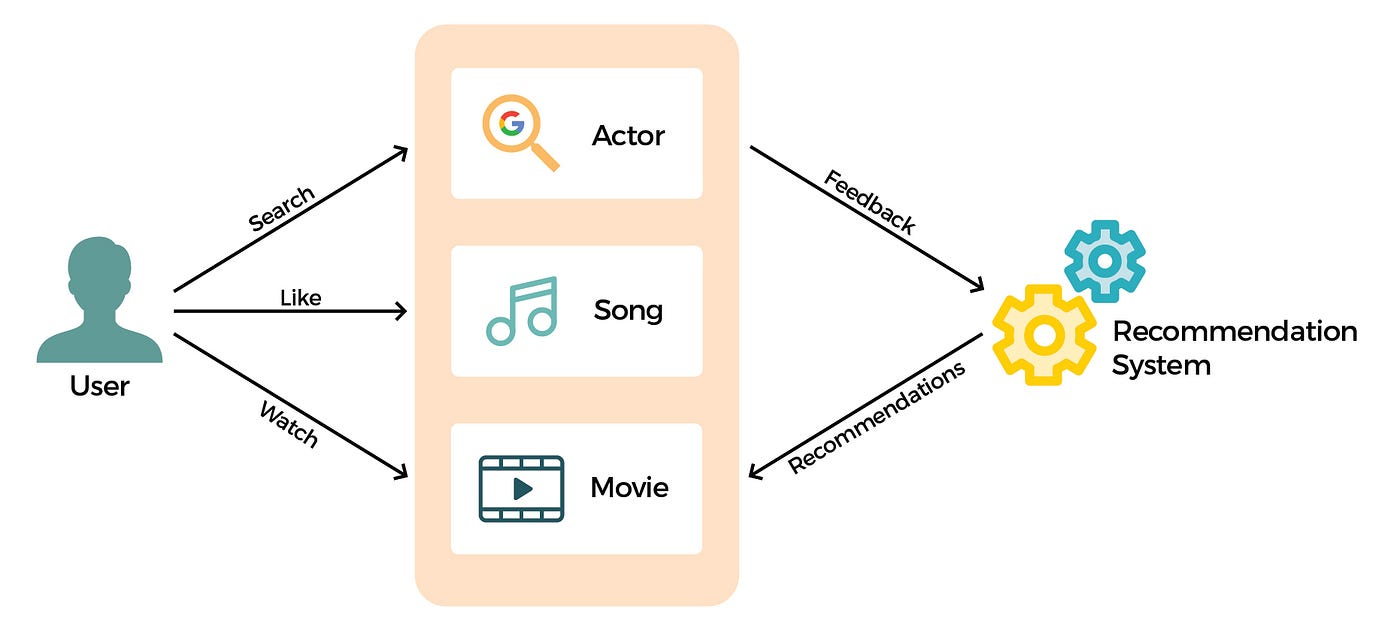
\includegraphics[height=0.2\textheight ,width=0.8\textwidth]{img/RecSys.png}
    \caption{Conceptual representation of a Recommender Systems}
\end{figure}

Recommender Systems are not perfect. They can suffer of several problems like:
\begin{itemize}
    \item \textbf{Cold Start Problem}: Because new users often have very few records in the system, it is hard to guess their preferences given the insufficient information\cite{ColdStart}
    \item \textbf{Data Sparsity}: Most users use the system but do not give rating for feedback to the system in a proper way.\cite{Sparsity}. In addition, in many real-word application we have thousand if not milion of user and item, so it's impossible to think that all user with interact with all item.
    \item \textbf{Scalability}: As the number of users and items increases, the computational complexity of recommendation algorithms can become a challenge. So we can divide scalability problems in two categories: 
    \begin{itemize}
        \item \textbf{Software Scalability}: There's a need to develop algorithms that can handle milions of users and items
        \item \textbf{Hardware Scalability}: There's a need to create systems with powerful hardware that can handle the computational cost in time and space
    \end{itemize}
    \item \textbf{Over Specialization }: Sometimes Recommender algorithms can "overfit" users' preferences, which lead to suggest items that are too similar to those already liked by the user not allowing him/her to discover new items that might be relevant
\end{itemize}


\subsection{Multimodal Recommender Systems}
Differently from classical recommendation approaches, multimodal recommendation exploits multimodal side information about items to enrich the interaction matrix, alleviating its sparsity, and to better understand the content to be recommended; these advantages, in general, lead to more accurate and precise recommendations\cite{Spillong}. We can think about different types of multimodal information: \textbf{Text} in natural language that can be used in every context, \textbf{Audio} for Music, \textbf{Images} for products such as clothes or fornitures, \textbf{Videos} for movies and so on.


The powerfulness of multimodal recommendation is given by the fact that different modalities can provide information about the same item from different perspectives. For example, in a movie recommender system, the textual description of a movie can provide information about its plot, screenshots from the film can provide visual clues about the style of photography and the type of film (animated, live-action, stop-motion, etc.)


Some DNN architectures known as \textbf{Encoders} are used to extract features from different modalities that can be used in different ways like:
\begin{itemize}
    \item \textbf{Concat}: Refers to the concatenation of multimodal features. \cite{ConcatFeature}
    \item \textbf{Fusion and attention}: Refers to the attention mechanisms (like self-attention) to combine multimodal features. \cite{Fusion}
    \item \textbf{GNNs}: They use Graph Neural Networks to model the relationships between items and users, incorporating multimodal features into the graph structure
\end{itemize}

\begin{figure}[H]
    \centering
    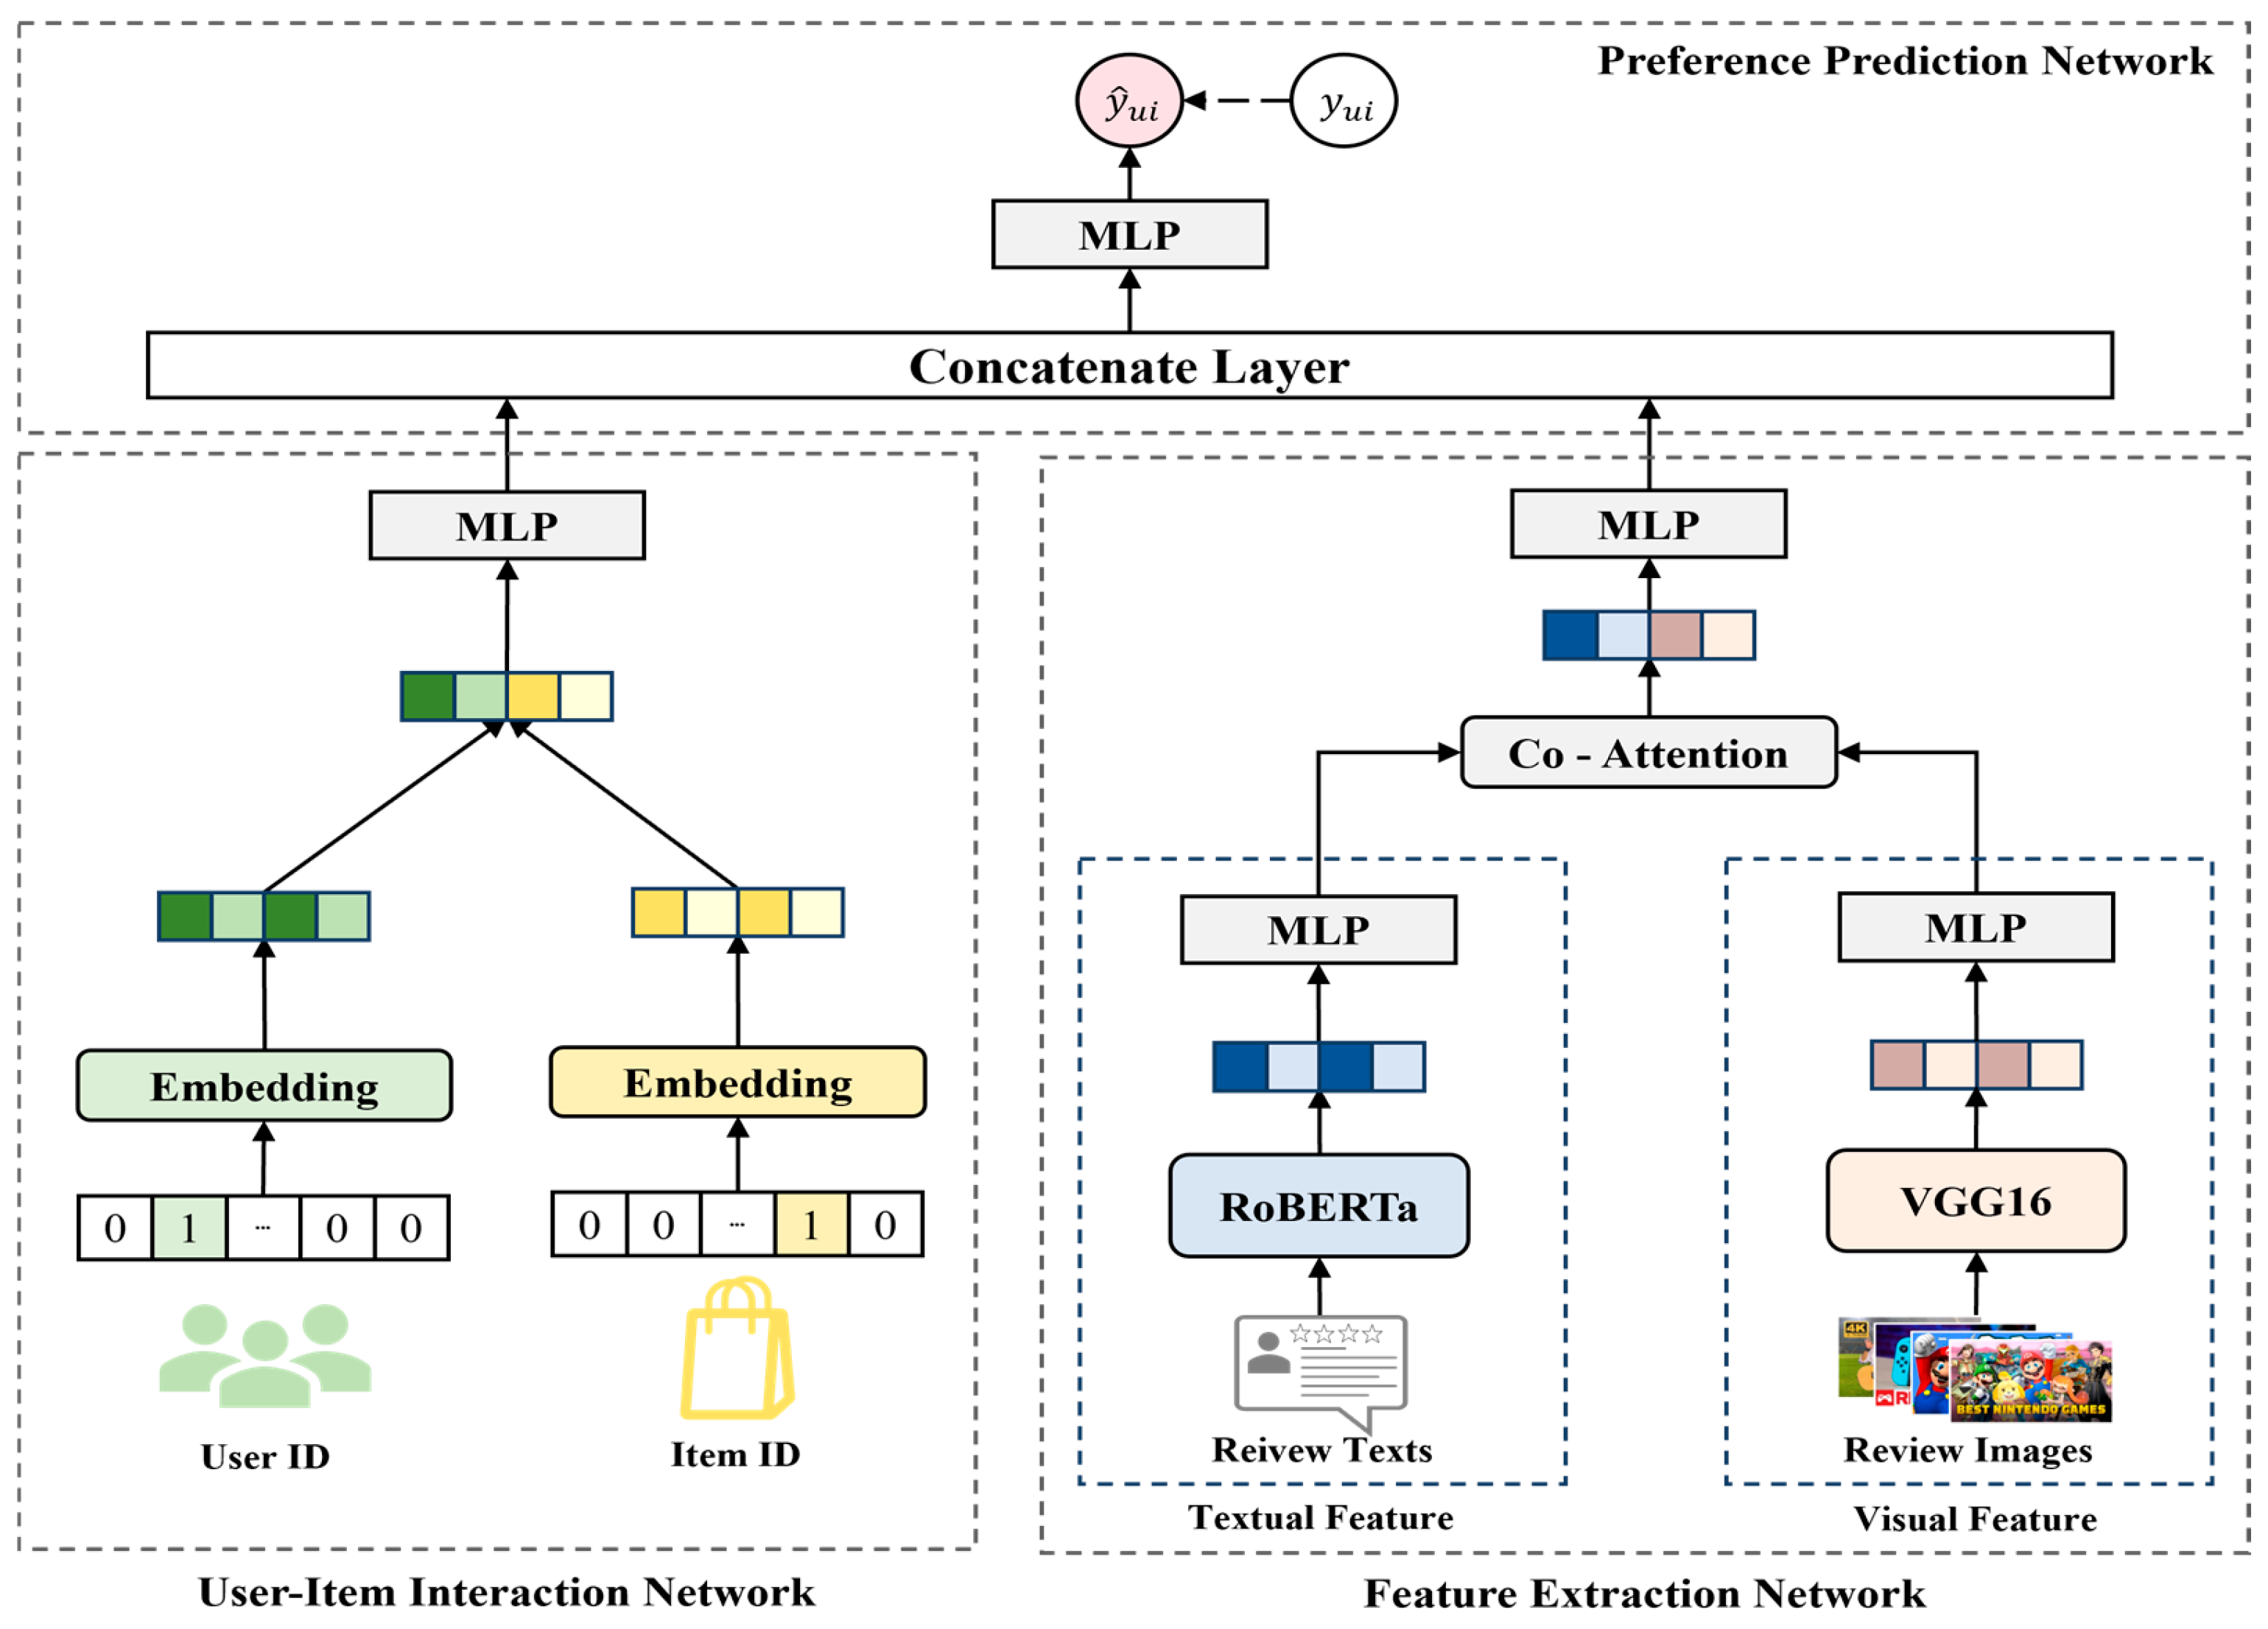
\includegraphics[height=0.5\textheight ,width=0.8\textwidth]{img/MMRec.png}
    \caption{Conceptual representation of a Multimodal Recommender Systems}
\end{figure}